From the given information, 
\begin{align}
\angle C = 90^{\degree}
\end{align}
Hence, 
\begin{align}
\vec{A}&=\myvec{0\\c\sin{B}}\\
              &=\myvec{0\\2.9}\\
\vec{B} &=\myvec{c\cos{B}\\0}\\
               &=\myvec {5.02294\\0}\\
\vec{C} &=\myvec{0\\0}
\end{align}
which are used to draw $\triangle ABC$ in Fig. \ref{triangle/20/fig:triangle ABC}.
%
\begin{figure}[!ht]
\centering
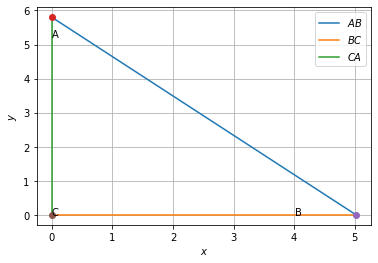
\includegraphics[width=\columnwidth]{solutions/triangle/20/Figure01.png}
\caption{$\triangle ABC$}
\label{triangle/20/fig:triangle ABC}
\end{figure}    
